\documentclass[tikz,border=10pt]{standalone}
\usetikzlibrary{calc}

\begin{document}
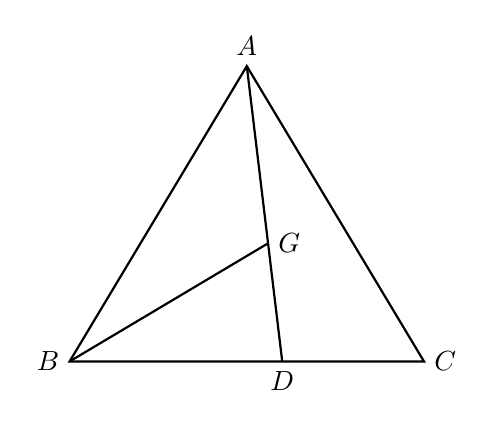
\begin{tikzpicture}[thick, scale=1.5]
    % 1. 定义坐标 (坐标可根据需求调整)
    \coordinate (B) at (0,0);
    \coordinate (C) at (3,0);
    \coordinate (A) at (1.5,2.5);
    % D 在 BC 上，取 BC 的中间偏右位置，模拟图中效果
    \coordinate (D) at (1.8,0); 
    % G 在 AD 上，取 AD 下方约 2/3 处
    \coordinate (G) at ($(A)!0.6!(D)$);

    % 2. 绘制主要三角形边界
    \draw (A) -- (B) -- (C) -- cycle;

    % 3. 绘制内部线段 AD 和 BG
    \draw (A) -- (D);
    \draw (B) -- (G);

    % 4. 标注点名
    \node[above] at (A) {$A$};
    \node[left]  at (B) {$B$};
    \node[right] at (C) {$C$};
    \node[below] at (D) {$D$};
    \node[right] at (G) {$G$};

\end{tikzpicture}
\end{document}